\documentclass[10pt,conference,letterpaper]{IEEEtran}
\IEEEoverridecommandlockouts
% The preceding line is only needed to identify funding in the first footnote. If that is unneeded, please comment it out.
\usepackage{cite}
\usepackage{amsmath,amssymb,amsfonts}
\usepackage{algorithmic}
\usepackage{graphicx}
\usepackage{textcomp}
\usepackage{xcolor}
\usepackage{booktabs}
\usepackage{array}
\usepackage{longtable}
\usepackage{multirow}
\usepackage{tabularx}
\usepackage{gensymb}
\usepackage[hyphens]{url}
\usepackage{xurl}
\usepackage{rotating}
\usepackage[euler]{textgreek}
\usepackage{placeins}
\usepackage{float}
\usepackage[colorlinks=true, allcolors=blue]{hyperref}

\def\BibTeX{{\rm B\kern-.05em{\sc i\kern-.025em b}\kern-.08em
    T\kern-.1667em\lower.7ex\hbox{E}\kern-.125emX}}

\newcommand{\todo}[1]{\textcolor{red}{\textbf{[TODO: #1]}}}

\newcommand{\takeaway}[1]{%
    \par\medskip
    \noindent\begingroup
    \setlength{\fboxsep}{7pt}%
    \setlength{\fboxrule}{0.6pt}%
    \fcolorbox{blue!40!black}{blue!4}{%
        \begin{minipage}{0.97\linewidth}
            \textcolor{blue!50!black}{\textbf{Takeaway.}} #1
        \end{minipage}%
    }%
    \endgroup
    \par\medskip
}

\begin{document}

\title{Evaluating MFU as a Portable Power Proxy for Energy-Aware LLM Simulation}


\author{\IEEEauthorblockN{Niklas Enskat}
\IEEEauthorblockA{\textit{Technische Universität Berlin} \\
enskat@campus.tu-berlin.de}
\and
\IEEEauthorblockN{Philipp Wiesner}
\IEEEauthorblockA{\textit{Technische Universität Berlin} \\
wiesner@tu-berlin.de}
}

\maketitle

\begin{abstract}
High-fidelity performance simulators are essential for designing and configuring efficient AI systems, yet today's tools lack the ability to predict power consumption.
This is due to a telemetry gap: simulators cannot access hardware-level utilization counters that are typically used for power modeling.
This work evaluates whether Model FLOPs Utilization (MFU)---an analytical, software-defined metric relating achieved throughput to peak hardware capability---can serve as a portable, software-defined predictor of GPU power for LLMs.
We benchmark almost 3000 training configurations across six GPUs, covering different model families, numerical precisions, batch sizes, and context-window lengths.
We find that a linear MFU-based power model fits every device in the compute-bound regime that dominates production LLM training.
The model class transfers across vendors and precisions; only the slope is hardware-specific, so supporting a new device requires just a one-shot calibration sweep.
Fitting per (GPU, dtype, batch size) cell drops the within-cell mean error from $\sim$10\,\% to $\sim$1\,\%, matching the cross-repeat measurement-noise floor.
\end{abstract}

\begin{IEEEkeywords}
GPU power modeling, energy-efficient AI, LLM simulation, MFU
\end{IEEEkeywords}

\section{Introduction}
The rapid progress of artificial intelligence (AI) has led to increasingly larger and more energy-demanding models~\cite{yang-2024B}. Training and deploying such models relies heavily on GPU-accelerated infrastructures, where GPUs have become the backbone of modern AI systems~\cite{jahanshahi-2020}.
As AI workloads contribute a growing share of global data-center electricity use~\cite{international-energy-agency-2025}, there is an intensifying need for energy-aware system design and predictive performance modeling~\cite{katsenou-2024, google-2024}.
High-fidelity simulators and analytical models are the primary tools used by researchers and system architects to explore "what-if" scenarios for future AI clusters, such as optimizing scheduling policies or evaluating different hardware parallelization strategies~\cite{agrawal2024vidur}.

However, predicting the power consumption of simulated AI workloads remains a fundamental challenge. Existing power models typically rely on hardware-level telemetry, such as GPU Utilization, which represents an aggregate measure of device activity reported by the hardware during execution~\cite{antarctica-2025, bridges-2016}.
While useful for operational monitoring, these metrics present a telemetry gap for simulation and performance modeling. 
First, hardware-defined counters are only available \emph{after} code execution on physical hardware, making them inaccessible during the design or simulation phase. 
Second, these metrics are vendor-specific (e.g., NVIDIA's NVML vs. AMD's ROCm), limiting the portability of derived power models across different providers or architectural generations.

A recently introduced yet already widely adopted performance metric for generative AI systems is Model FLOPs Utilization (MFU)~\cite{chowdhery-2023}. 
Unlike hardware counters, MFU is an analytical metric that relates observed throughput to the theoretical peak compute capacity required per token. 
Because MFU is derived from the model structure and high-level execution parameters, it can be calculated by simulators (e.g., Microsoft's Vidur~\cite{agrawal-2025}) without access to physical hardware. 
While MFU has been proposed as a candidate input for power modeling in these settings~\cite{ozcan-2025}, its predictive value and robustness across diverse hardware have not been systematically evaluated.

This paper investigates whether MFU can serve as a reliable, portable, and software-defined proxy for GPU power consumption.
For LLM training, which is predominantly compute-bound, MFU captures the compute saturation that drives power consumption.
We validate MFU against ground-truth hardware measurements, providing a portable methodology for energy-aware simulation without vendor-specific telemetry.

To do so, we build a cross-architectural benchmarking framework and execute a controlled training sweep on \emph{six} accelerators spanning two vendors and four hardware tiers (NVIDIA A100, L40, L4, Quadro RTX~5000, RTX~4070~Ti, and AMD MI210).
The sweep crosses three model families (Qwen2.5, GPT-2, DialoGPT), three numerical precisions (fp32, fp16, bf16), seven batch sizes (1--128), and two context-window lengths (512, 2048~tokens), yielding 504 configurations per device, each repeated four times with telemetry sampled until statistical convergence.
For every configuration, we record MFU, vendor-reported GPU~Utilization, and GPU power, and use this dataset to evaluate MFU and GPU~Utilization as predictors of power across hardware platforms and workload regimes.
We use internal GPU telemetry (NVML on NVIDIA, ROCm on AMD) as the reference power signal throughout. Appendix~\ref{sec:power-validation} documents agreement with external wall-power measurements for two devices.

Our key findings are:
\begin{itemize}
    \item A linear MFU-power model fits every GPU we measure ($R^2$ 0.68--0.84), including AMD MI210 where vendor-reported GPU~Utilization is a binary activity flag and admits no linear fit at all.
    \item The slope is hardware-specific (MFU is peak-FLOPS-normalized), but the model \emph{class} transfers across vendors and precision modes, so supporting a new accelerator needs only a one-shot per-GPU calibration sweep.
    \item Conditioning a separate linear fit per (GPU, dtype, batch size) cell collapses within-cell MAPE from $\sim$10\,\% pooled to $\sim$1\,\%, which is statistically indistinguishable from the cross-repeat measurement-noise floor. The practical recipe for an MFU-based power proxy is therefore to condition on these three axes and on nothing else.
    \item At batch~1, MFU collapses below 1.3\,\% while power stays at $\sim$60\,\% of the batch-128 level. Further-out memory-bound regimes need a complementary memory-bandwidth signal.
\end{itemize}

Our benchmarking pipeline and data are publicly available: \url{https://github.com/dos-group/gpu_power_benchmark}.


\section{Performance and Power Metrics for GPUs}\label{Background}
Modern LLM training workloads impose sustained high computational demand and correspondingly high GPU power draw, so understanding how workload performance metrics relate to energy behavior is central to both efficient operation and predictive modeling.
Floating-point operations per second (FLOPS) are the conventional starting point for describing GPU compute capability, with vendors reporting theoretical peaks under idealized conditions. Real training workloads rarely approach these peaks because of memory effects, scheduling overhead, communication latency, and kernel structure, so the relevant practical question is which fraction of peak compute a workload actually realizes and how that fraction relates to power.
The remainder of this section reviews two utilization metrics commonly used to answer this question (\S\ref{sec:bg-gpu-util},~\S\ref{sec:bg-mfu}) and then outlines how GPU power is measured and estimated in practice (\S\ref{sec:bg-power}).

\subsection{GPU Utilization}\label{sec:bg-gpu-util}
GPU Utilization is commonly reported via tools such as \texttt{nvidia-smi} or \texttt{rocm-smi} and is typically defined as the fraction of time during which the GPU is actively executing kernels within a sampling interval~\cite{cornelius-2025, nvidia-no-dateA}. It is widely used for operational monitoring due to its simplicity and availability.
However, GPU~Utilization is a time-based activity metric rather than a measure of compute-efficiency. High utilization may correspond to memory-bound execution, synchronization overhead, or stalled kernels, without implying productive throughput. It is also a vendor-defined counter whose semantics differ across vendors and architectural generations, so equal values can correspond to substantially different throughput and power behavior.
These characteristics limit GPU~Utilization as a universal efficiency metric and raise the question about its suitability as a predictor of energy consumption.
It is nevertheless frequently used as an input to GPU power models~\cite{antarctica-2025, bridges-2016}.

\subsection{Model FLOPs Utilization (MFU)}\label{sec:bg-mfu}
MFU relates observed throughput (tokens per second) to the theoretical compute required per token, normalized by the peak compute capacity of the GPU for the specific numerical precision (dtype) used.
Unlike a hardware-defined activity counter, MFU is derived purely from the model architecture and measured throughput, making it a software-defined metric that can be computed inside a simulator without access to physical hardware.
Concretely, MFU~\cite{chowdhery-2023,ray-2025} is defined as
\begin{equation*}
    \text{MFU} = \frac{\text{Tokens/s} \cdot C_{\text{req}}}{\text{FLOPS}_{\text{peak}}},
\end{equation*}
where $C_{\text{req}}$ is the floating-point \emph{operation count} required for a forward and backward pass of a single token, and $\text{FLOPS}_{\text{peak}}$ is the theoretical peak throughput (operations per second) for the used precision and hardware generation.
For dense transformer models, $C_{\text{req}}$ is commonly approximated as
\begin{equation*}
    C_{\text{req}} = 6N + 12\,L_{\text{num}} H_{\text{num}} Q_{\text{dim}} T_{\text{seq}},
\end{equation*}
where $N$ is the number of model parameters, $L_{\text{num}}$ the number of layers, $H_{\text{num}}$ the number of attention heads, $Q_{\text{dim}}$ the head dimension, and $T_{\text{seq}}$ the sequence length~\cite{chowdhery-2023}.
In practice the exact operation count is more involved due to architectural and implementation details, so we use the integrated profiler CalFLOPS~\cite{calflops} to obtain $C_{\text{req}}$ directly.

Whether MFU can act as a reliable predictor of GPU power consumption depends on the execution regime.
In \textit{compute-bound} regions, performance is limited by arithmetic throughput, which MFU captures by construction.
In \textit{memory-bound} regions, the bottleneck shifts to data transfer between memory and processors. GPU~Utilization may remain high while MFU drops, and the linear MFU--power relationship is no longer expected to hold.
Because MFU reflects effective training progress rather than total executed operations, it is also less sensitive to implementation-specific recomputation effects than counter-based metrics.
This makes MFU an attractive abstraction for comparing training efficiency across devices and configurations.
Yet, as a power predictor, it has not been systematically validated, motivating the study in the remainder of this paper.

\subsection{GPU Power Measurement and Estimation}\label{sec:bg-power}
Modern data-center and workstation GPUs expose on-board power telemetry through vendor management interfaces (NVML on NVIDIA, ROCm SMI on AMD), reporting board-level power at sub-second granularity~\cite{weakley-2025}. These signals are convenient and ubiquitous, and we use them as the ground-truth power signal throughout this study. Appendix~\ref{sec:power-validation} validates them against external node-level wall-power measurements for two of our devices.
External hardware power meters can provide reference measurements at higher accuracy and at component or node level~\cite{yang-2024A, jay-2023}, but their deployment requires dedicated instrumentation and does not scale easily to large clusters.
Where direct measurement is impractical (most prominently in simulation and design-space exploration) analytical and statistical models estimate power from hardware activity counters and performance metrics~\cite{lang-2013}.
Such models depend on calibration data and typically rely on architecture-specific telemetry, which limits their portability across vendors and generations~\cite{yang-2024A} and prevents their use in simulators that have no hardware counters to read in the first place. This portability gap is exactly what an MFU-based power model aims to close.

\section{Experimental Framework}\label{methodology}
To validate MFU as a simulation proxy, we develop a cross-architectural benchmarking framework that maps high-level model parameters to empirical power consumption.

\subsection{Workload Selection and Execution}\label{exp. design}
We conduct controlled experiments across multiple model scales, batch sizes, precision modes, and context window lengths on diverse GPU platforms. 
For each configuration, we record hardware telemetry signals until statistical convergence is reached to ensure stable estimates.
We define \textit{convergence} as the point where the 95\,\% confidence-interval half-width of both MFU and GPU~Utilization falls within 5\,\% of their running mean (i.e.\ $1.96 \cdot \text{SEM}/\bar{x} \le 0.05$), evaluated cumulatively after a minimum of 50 sampling intervals (1\,s each) and capped at 500 intervals to bound run length. Power is sampled jointly but is not part of the stopping rule, since it is the smoother of the three signals; once both predictor signals are stable, power is stable by extension. 
Each configuration is preceded by 5 warmup training steps that are excluded from telemetry, allowing the GPU to reach steady-state compute behavior before recording begins; configurations are separated by a 2\,s cooldown interval to bound thermal carryover between runs.
This design enables correlation and regression analysis of utilization metrics as predictors of GPU power consumption across hardware generations.

To support reproducible data collection, we implement a Python-based benchmarking framework that automates configuration sweeps, workload execution, telemetry sampling, and convergence control. Experimental parameters are defined and expanded into run configurations through Hydra~\cite{Yadan2019Hydra}, ensuring traceability and reproducibility.

\subsection{Search Space and Software}\label{sec:setup}
We sweep training across the following axes:
\begin{itemize}
    \item \textbf{6 GPUs:} NVIDIA A100, L40, L4, Quadro RTX 5000, RTX 4070 Ti, and AMD MI210.
    \item \textbf{3 model families} (Qwen2.5, GPT-2, DialoGPT), with sizes matched to GPU tier:
          commodity (RTX 4070 Ti, Quadro): 0.5B\,/\,124M\,/\,medium;
          mid (L40, L4): 1.5B\,/\,GPT-2-XL\,/\,large;
          high-end (A100, MI210): 3B\,/\,GPT-2-XL\,/\,large.
    \item \textbf{3 numerical precisions:} float32, float16, bfloat16\footnote{The Quadro RTX 5000 lacks hardware bfloat16 support.}.
    \item \textbf{7 batch sizes:} 1, 4, 8, 16, 32, 64, 128.
    \item \textbf{2 context windows:} 512 and 2048 tokens.
\end{itemize}
The cross product gives 126 workload configurations per GPU (84 on the Quadro 5000).
Each is repeated four times.
Optimizer, learning rate, attention implementation, sampling interval (1\,s), and single-GPU execution are held constant.
Gradient scaling is disabled for consistency across precisions.

Our software stack uses PyTorch~\cite{paszke2019pytorch} and Hugging Face Transformers~\cite{wolf2019huggingface0s} for model execution, NVML\footnote{\url{https://developer.nvidia.com/management-library-nvml}} on NVIDIA and ROCm\footnote{\url{https://www.amd.com/en/products/software/rocm.html}} on AMD~\cite{weakley-2025} for telemetry, and CalFLOPS~\cite{calflops} for FLOP profiling.
Software-reported GPU power is read from on-board sensors via NVML/ROCm. Two systems are additionally instrumented with external node-level meters (Appendix~\ref{sec:power-validation}).

\section{Experiments}\label{results}
This section evaluates how well MFU and GPU Utilization predict GPU power consumption across hardware platforms and workload configurations. We report predictor--power relationships, error characteristics, and sensitivity to experimental variables.

\subsection{A Linear MFU-Based Power Model Fits Every GPU}\label{Predictor Performance}
A linear model relating MFU to internal GPU power fits every device we measured, including the AMD MI210 where vendor utilization gives no usable signal at all. Table~\ref{tab:per_gpu_mfu_power} reports the per-GPU pooled fit alongside the GPU~Utilization counterpart for context, with 95\,\% bootstrap confidence intervals (2000 resamples over configurations).

The pooled MFU fits explain 68--84\,\% of variance in internal power across NVIDIA devices, and 77\,\% on AMD MI210. Mean absolute percentage errors (MAPE) range from 7.8\,\% on the L40 to 13.7\,\% on MI210. This is sufficient precision for the ``what-if'' energy comparisons targeted by training simulators. GPU Utilization fits are tighter than MFU on NVIDIA hardware (0.67--0.87) but \emph{not fittable} on MI210: ROCm reports utilization from the \texttt{GRBM\_COUNT} counter, which acts as a binary activity flag rather than a throughput percentage and saturates at 100\,\% under any sustained training workload. MFU is therefore the only predictor of the two that yields a fittable model across all five devices.

\begin{table}[t]
    \centering
    \caption{Per-GPU linear MFU-based power fits over all configurations. Errors are 95\,\% bootstrap CIs.}
    \label{tab:per_gpu_mfu_power}
    \begin{tabular}{lccc}
        \toprule
        \textbf{GPU} & \textbf{MFU $R^2$} & \textbf{MFU MAPE} & \textbf{GPU Util $R^2$} \\
        \midrule
        NVIDIA A100        & $0.74 \pm 0.03$ & $11.0 \pm 0.7$\,\%           & $0.87$ \\
        NVIDIA L40         & $0.80 \pm 0.03$ & $\phantom{0}7.8 \pm 0.5$\,\% & $0.82$ \\
        NVIDIA Quadro 5000 & $0.84 \pm 0.02$ & $12.5 \pm 1.4$\,\%           & $0.85$ \\
        NVIDIA RTX 4070 Ti & $0.68 \pm 0.06$ & $12.5 \pm 1.1$\,\%           & $0.67$ \\
        AMD MI210          & $0.77 \pm 0.05$ & $13.7 \pm 0.9$\,\%           & ---     \\
        \bottomrule
    \end{tabular}
\end{table}

\begin{figure}[t]
    \centering
    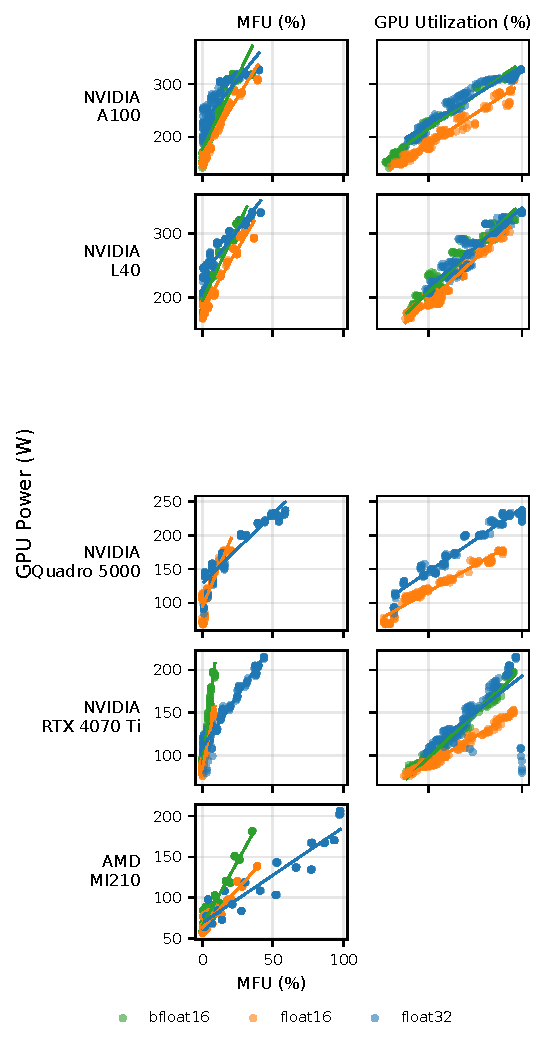
\includegraphics[width=\columnwidth]{figures/predictor_vs_power.pdf}
    \caption{MFU and GPU~Utilization versus internal GPU power. The MI210 appears only in the MFU panel because its GPU~Utilization signal is effectively binary (Section~\ref{Predictor Performance}).}
    \label{fig:Predictors across DTypes}
\end{figure}

\paragraph{Slopes are hardware-specific by construction.}
The fitted slopes of the MFU-based power model range from 1.21\,W per percent of MFU on the MI210 to 4.49 on the A100. This 3.7$\times$ spread mirrors the spread in peak per-precision FLOPS across these devices. Because MFU normalizes throughput by peak FLOPS, equal MFU values correspond to different raw arithmetic work on different chips, and power scales with raw arithmetic work. The portability claim is therefore that the \emph{model class} (linear, MFU-based) transfers across vendors and precision modes, not that a single slope does. A simulator targeting a new device needs a one-shot per-GPU calibration sweep, after which power follows from MFU alone. This is precisely the input simulators already produce as an analytical metric~\cite{agrawal-2025,ozcan-2025}.

\paragraph{Within-cell tightness corroborates a mechanistic relationship.}
Holding numerical precision and batch size fixed, MFU explains 98\,\% of power variance on the MI210 (median $R^2 = 0.997$ across 21 cells; mean $0.980$, std $0.038$). The corresponding NVIDIA medians range from $0.89$ (RTX 4070 Ti) to $0.98$ (A100, Quadro 5000); their lower means and higher dispersion are driven by saturation cells at the largest batch sizes, where both MFU and power vary by less than 3\,\% and $R^2$ is dominated by sub-percent measurement noise (Section~\ref{Relationship Across Variables}). The pooled $R^2$ values in Table~\ref{tab:per_gpu_mfu_power} are regime-averaged mixtures rather than evidence of a noisy underlying relationship. Figure~\ref{fig:Predictors across DTypes} shows the underlying scatter: within each dtype, power scales near-linearly with MFU on every device, with per-dtype slopes that reflect the peak-FLOPS spread noted above.

\takeaway{A linear MFU-based power model fits every device we measured, including the AMD~MI210 where GPU~Utilization is a binary activity flag and admits no linear fit. The \emph{model class} transfers across vendors and precisions. Howeverm, the per-device \emph{slope} does not, because MFU normalizes by peak FLOPS. Supporting a new accelerator therefore needs only a one-shot per-GPU calibration sweep.}

\subsection{Conditioning the Model}\label{Relationship Across Variables}
Section~\ref{Predictor Performance} established that a linear MFU-based power model fits every GPU. Two questions remain: which workload variables shift the slope of that fit, and how far does conditioning on them reduce prediction error before the data themselves run out of signal?

\paragraph{Regime variables.}
Of the workload axes we vary, only \emph{numerical precision} and \emph{batch size} materially shift the MFU-power relationship. Figure~\ref{fig:Predictors across DTypes} shows the per-dtype OLS fits: reduced-precision formats shift the predictor distributions and change the slope of the line, with MFU exhibiting stronger dtype-dependent scaling than GPU~Utilization. This is expected, since MFU is normalized against a dtype-specific peak FLOPS rate. Figure~\ref{fig:Predictors vs Batch} resolves the batch dimension: MFU rises smoothly from $\sim$1\,\% at batch~1 to 28--44\,\% at batch~128, tracking arithmetic throughput. GPU~Utilization sits at 40--55\,\% already at batch~1 and saturates near 90\,\% well before MFU does. On the MI210, GPU~Utilization is pinned at 100\,\% across every batch size: the ROCm \texttt{GRBM\_COUNT}-based signal flags activity, not throughput. Context window length (512 versus 2048 tokens) has no measurable effect on either predictor or on power.

\begin{figure}[t]
    \centering
    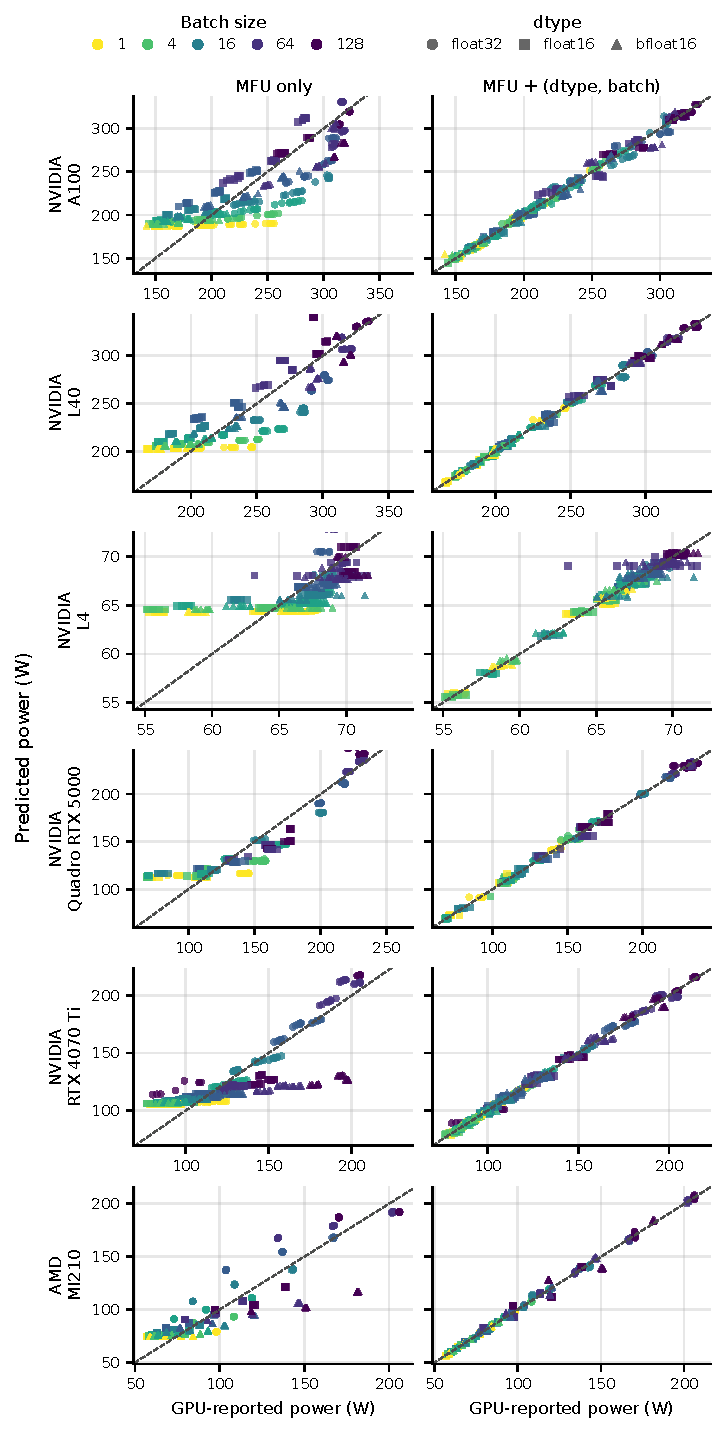
\includegraphics[width=\columnwidth]{figures/predicted_vs_measured_power.pdf}
    \caption{Predicted versus measured GPU power. Batch-1 configurations (yellow) cluster off the diagonal because the memory-bound regime breaks the single-slope fit (Section~\ref{sec:failure-modes}). Under (dtype, batch)-conditioned models predictions collapse onto the diagonal across batch sizes and dtypes.}
    \label{fig:pred_vs_meas_power}
\end{figure}

\begin{figure}[t]
    \centering
    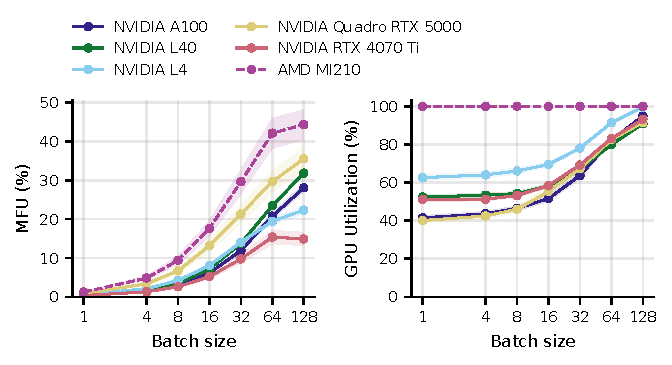
\includegraphics[width=\columnwidth]{figures/predictors_vs_batch.pdf}
    \caption{Per-GPU mean MFU (left) and GPU~Utilization (right) as a function of batch size (log scale). MFU tracks arithmetic throughput and ramps smoothly with batch on every device; GPU~Utilization rises shallowly on NVIDIA and pins at 100\,\% on the MI210 from batch~1 onward, reflecting its activity-flag semantics. Shaded bands are $\pm$1\,SEM across configurations.}
    \label{fig:Predictors vs Batch}
\end{figure}

\paragraph{Conditioning lift.}
Fitting a separate linear MFU-power model per (dtype, batch) cell collapses the prediction error from $\sim$10\,\% pooled across the search grid to $\sim$1\,\% within each cell, on every device. Figure~\ref{fig:Prediction Error Figure} (bottom) shows the resulting error distributions. Figure~\ref{fig:pred_vs_meas_power} (bottom) shows predicted versus measured power hugging the diagonal across both batch sizes and dtypes. The tail behavior of the pooled fit is informative on its own: GPU~Utilization's pooled 95th-percentile error stays below 26\,\% on every NVIDIA device, while MFU can exceed 30\,\% (worst case 57.9\,\% on the Quadro~5000), with the heavier-tail outliers clustering under reduced precision. The RTX~4070~Ti reverses this ordering: both predictors fit it worst overall, reflecting the workstation environment in which it was measured (Section~\ref{Limitations}).

\begin{figure*}[t]
    \centering
    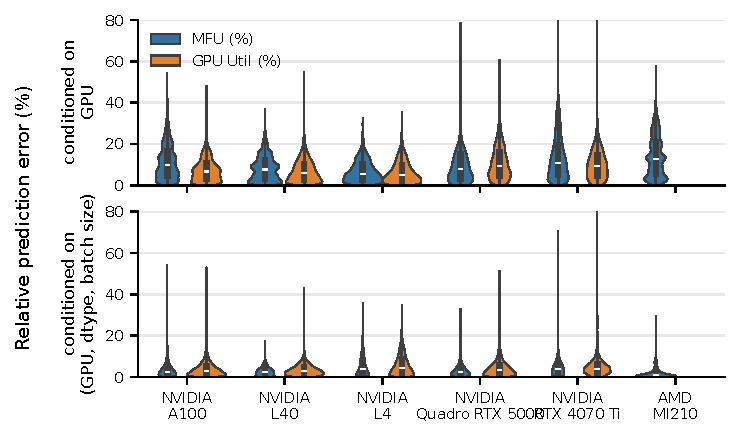
\includegraphics[width=\textwidth]{figures/prediction_error.pdf}
    \caption{Distribution of per-sample absolute relative error ($|\text{actual} - \text{predicted}| / \text{actual}$) for linear regressions from MFU or GPU Utilization to power draw, across all tested hardware.
             Conditioning on (dtype, batch size) substantially reduces error for both predictors on all devices.}
    \label{fig:Prediction Error Figure}
\end{figure*}

\paragraph{The conditioned model is at the data limit.}
The $\sim$1\,\% MAPE quoted above is an in-sample number. Whether the remaining error is model misspecification or measurement noise is a separate question. Our experimental design lets us answer it directly: each of the 504 (336 on the Quadro~5000) per-GPU configurations is measured across four independent repeats separated by large time gaps in the raw stream. The cross-repeat standard deviation of mean power therefore bounds any predictor's achievable accuracy. Table~\ref{tab:noise_floor} compares the pooled per-GPU MFU model's residual SD, the (dtype, batch)-conditioned model's residual SD, and the cross-repeat measurement-noise SD, each as a percentage of the GPU's mean power. Conditioning cuts the pooled residual by 5--6$\times$ on every device, and on every NVIDIA GPU the conditioned residual is within 1.1--2.7$\times$ of the noise floor. On the Quadro~5000 and RTX~4070~Ti it is statistically indistinguishable from it. The MI210 is the lone outlier in relative terms: its AMD power telemetry is unusually quiet (cross-repeat SD of 0.23\,\% against $\geq$0.45\,\% on every NVIDIA device), but its conditioned residual is in line with the rest of the fleet in absolute terms.

\begin{table}[t]
\centering
\caption{Residual standard deviation of the MFU power model (pooled and (dtype, batch)-conditioned) versus the cross-repeat measurement-noise floor, each as a percentage of mean GPU power. The conditioned model is within a small factor of the noise floor on every NVIDIA GPU; the MI210's AMD power telemetry is unusually quiet, leaving visible model headroom in relative but not absolute terms.}
\label{tab:noise_floor}
\small
\setlength{\tabcolsep}{4pt}
\renewcommand{\arraystretch}{1.15}
\begin{tabular}{lccc}
    \toprule
    \textbf{GPU} & \textbf{Pooled MFU} & \textbf{+ (dtype, batch)} & \textbf{Repeat noise} \\
    \midrule
        NVIDIA A100 & 12.49\,\% & 2.13\,\% & 1.48\,\% \\
        NVIDIA L40 & 9.01\,\% & 1.29\,\% & 0.45\,\% \\
        NVIDIA Quadro 5000 & 12.79\,\% & 1.95\,\% & 1.73\,\% \\
        NVIDIA RTX 4070 Ti & 16.44\,\% & 2.21\,\% & 2.16\,\% \\
        AMD MI210 & 17.43\,\% & 2.81\,\% & 0.23\,\% \\
    \bottomrule
\end{tabular}
\end{table}


\takeaway{Within the compute-bound regime, conditioning the MFU power model on dtype and batch size --- and on nothing else --- reduces MAPE from $\sim$10\,\% pooled to $\sim$1\,\% per cell, and the resulting residual matches the cross-repeat measurement noise on every NVIDIA GPU. The remaining error is sampling noise, not model misspecification: a more elaborate predictor would yield no measurable accuracy gain.}

\subsection{MFU Underestimates Power in Memory-Bound Regimes}\label{sec:failure-modes}
MFU normalizes throughput by peak FLOPS, so any workload bottlenecked on memory bandwidth rather than arithmetic will execute with low MFU even when power and GPU~Utilization remain high. Our existing search grid already brackets this boundary at its low-arithmetic-intensity end. The signature is visible in Figure~\ref{fig:pred_vs_meas_power} (top): batch~1 configurations (yellow) sit as a flat horizontal band well off the diagonal --- the pooled MFU model predicts essentially the intercept for every batch~1 point, while their measured power spans more than 100\,W. Table~\ref{tab:batch1_memory_bound} quantifies the gap: MFU collapses by 35--75$\times$ across the five GPUs from batch~1 to batch~128, but power changes by only $1.6$--$2.0\times$. At batch~1, every GPU runs below 1.3\,\% MFU while drawing 50--65\,\% of its batch-128 power. The slopes of Section~\ref{Predictor Performance} therefore extrapolate downward through this regime and substantially under-predict power, with a 70--120\,W absolute error on the data-center cards.

\begin{table}[t]
    \centering
    \caption{Batch-1 (memory-bound) versus batch-128 (compute-bound), averaged over models, precisions, and context windows.}
    \label{tab:batch1_memory_bound}
    \small
    \setlength{\tabcolsep}{4pt}
    \begin{tabular}{lcccc}
        \toprule
        \textbf{GPU} & $\mathbf{MFU_{1}}$ & $\mathbf{MFU_{128}}$ & $\mathbf{P_{1}}$\,(W) & $\mathbf{P_{128}}$\,(W) \\
        \midrule
        NVIDIA A100        & 0.4\,\% & 28.1\,\% & 189 & 307 \\
        NVIDIA L40         & 0.4\,\% & 31.8\,\% & 200 & 315 \\
        NVIDIA Quadro 5000 & 0.8\,\% & 35.5\,\% & 111 & 201 \\
        NVIDIA RTX 4070 Ti & 0.3\,\% & 14.9\,\% & \phantom{0}97 & 169 \\
        AMD MI210          & 1.2\,\% & 44.3\,\% & \phantom{0}72 & 148 \\
        \bottomrule
    \end{tabular}
\end{table}

Batch~1 with 2048-token contexts is the smallest-arithmetic-intensity workload in our sweep, but still well inside the LLM-training scope. Workloads with even lower arithmetic intensity (decode-style inference, or training with very small models at very long contexts) would extrapolate further outside the regime where a linear MFU-based power model is informative. A quantitative characterization of that extrapolation, ideally paired with a complementary memory-bandwidth signal, is left to future work.

\takeaway{The MFU-based power model holds inside the compute-bound regime that dominates production LLM training. At its low-arithmetic-intensity edge (batch~1) MFU already collapses below 1.3\,\% while power stays at $\sim$60\,\% of the batch-128 level. A single linear slope cannot serve both regimes, and very-low-batch or decode-style workloads need a complementary memory-bandwidth signal.}


\section{Limitations}\label{Limitations}
While the experimental design of this study enables consistent comparisons across predictors of and hardware platforms, several limitations constrain the generalizability of the findings.

The study evaluates mostly NVIDIA GPUs, spanning from consumer-level to data-center-level accelerators. This selection provides a meaningful contrast in architectural tier and deployment setting, but does not capture behavior across multiple accelerator generations or system designs with substantially different power management policies. Results therefore may not generalize to other accelerators with different workload behavior.
Additionally, the RTX 4070 Ti was measured in a workstation environment, rather than in a dedicated compute node, which introduced uncontrolled background activity and runtime interference. While this setup provides a realistic depiction of consumer-grade deployment conditions, it increases result variability and may reduce comparability with more controlled systems.



\section{Related Work}\label{related work}
GPU power consumption is closely tied to workload-dependent hardware activity. Previous work has analyzed this relationship through hardware-exposed utilization metrics, telemetry at system scale, and compute-centric abstractions. However, existing approaches often rely on vendor-specific instrumentation, limiting portability across architectures and preventing direct use in performance modeling or simulation frameworks.

\subsection{Utilization Metrics and Power Correlation}
Elvinger et al.~\cite{elvinger-2025} analyze GPU utilization under kernel colocation and show that coarse metrics such as achieved occupancy fail to capture resource interference across shared architectural components. Instead, more fine-grained indicators such as instructions per cycle (IPC) and pipeline utilization provide more expressive insight into hardware behavior. Their work demonstrates that utilization metrics differ significantly in their explanatory power, and that broad vendor-defined counters may obscure relevant activity. However, their study focuses on performance interference and does not examine energy behavior.

Utilization and energy is bridged more directly by Islam et al.~\cite{islam-2024}, as they present a data-driven characterization of GPU kernels using NVIDIA's NVML and CUPTI interfaces. They show that streaming multiprocessors (SM) activity correlates strongly with power draw during compute phases, therefore establishing an empirical link between hardware utilization and energy consumption. While this work confirms that utilization signals are predictive of power at kernel granularity, the proposed methodology depends on vendor-specific, hardware-exposed counters whose semantics and availability vary across architectures. As a result, such metrics are difficult to transfer across devices and cannot be used in simulation environments where hardware telemetry is unavailable.
Similarly, AccelWattch~\cite{kandiah2021accelwattch} models GPU power from microarchitectural activity counters with high fidelity, but requires architecture-specific instrumentation that is unavailable in high-level simulation frameworks.

At the system scale, Fernandez et al.~\cite{fernandez-2024} study distributed transformer training and observe diminishing returns due to communication overhead. Their analysis incorporates MFU as a performance indicator and highlights that compute efficiency degrades under scaling regimes. Although MFU is primarily treated as a throughput metric, this work suggests that compute-centric measures provide a stable abstraction of workload efficiency across hardware configurations.

\subsection{Compute-centric Energy Abstractions}
An alternative approach models energy consumption from computational cost. Desislavov et al.~\cite{desislavov-2023} estimate inference energy demand by combining model FLOPS with FLOPS-per-Watt efficiency figures across hardware generations. Their analysis highlights long-term trends in compute growth and hardware efficiency improvements. This illustrates the appeal of compute-based abstractions as FLOPS are independent from hardware, derivable from model structure, and independent of vendor instrumentation. However, their estimates rely largely on theoretical efficiency assumptions rather than empirical system-level power measurements, leaving the predictive accuracy of FLOPS-based abstractions uncertain in practical workloads.

\subsection{Portability Challenges in Simulation-Based Modeling}
The limitations of hardware-dependent utilization metrics become particularly evident in performance modeling and simulation frameworks. Systems such as VIDUR, introduced by Agrawal et al.~\cite{agrawal-2025}, model LLM execution based on workload structure and parallelization strategies without exposing hardware-level utilization counters. Consequently, vendor-defined metrics such as GPU Utilization or SM activity cannot be incorporated into the modeling process.

To enable energy estimation, Özcan et al.~\cite{ozcan-2025} extend this simulation framework with utilization-derived power models that infer energy demand from execution characteristics. However, these approaches rely on implicit utilization proxies rather than explicitly defined, portable metrics. Since hardware-exposed counters are unavailable in simulation, the choice of utilization abstraction remains underspecified.

\section{Conclusion}\label{Conclusion}
We evaluated MFU as a portable, software-defined power proxy for LLM training simulation across five GPUs from NVIDIA and AMD. A linear MFU-based power model fits every device (per-GPU $R^2$ 0.68--0.84), including the AMD MI210 where GPU Utilization is a binary activity flag and admits no linear fit at all. The fitted slope is hardware-specific by construction, since MFU is normalized by per-GPU peak FLOPS. The model class itself transfers, so a simulator targeting a new device needs only a one-shot per-GPU calibration. Within the compute-bound regime, dtype and batch size are the workload variables that shift the slope; context window length can be ignored. At the low-arithmetic-intensity edge of LLM training (batch~1), MFU collapses below 1.3\,\% on every GPU while power stays near 60\,\% of the batch-128 level, marking the boundary beyond which a complementary memory-bandwidth signal is required.

Because MFU is already exposed as an analytical output by performance simulators such as Vidur~\cite{agrawal-2025}, an MFU-based power model closes the simulator-to-energy loop without requiring a separate hardware-counter model. This delivers vendor-portable energy estimation for what-if studies in compute-bound LLM training, without ever needing access to physical hardware telemetry.

\appendices
\section{Power Measurement Validation}\label{sec:power-validation}
\begin{figure}[hbt!]
    \centering
    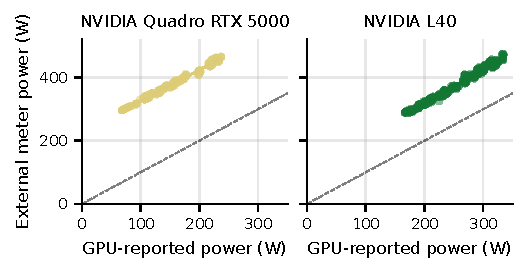
\includegraphics[width=\columnwidth]{figures/external_vs_internal_power.pdf}
    \caption{Validating ground-truth reliability: Internal GPU-reported vs. external hardware-based power measurements for NVIDIA L40 and Quadro RTX 5000. Each color represents a distinct GPU model with its corresponding linear fit.}
    \label{fig:Ex. vs Int. Power by Hardware}
\end{figure}
Reliable power measurements are a prerequisite for utilization-based modeling.
For the Quadro RTX 5000 and NVIDIA L40, we recorded external node-level power readings and compared them against internal GPU power.
As shown in Figure~\ref{fig:Ex. vs Int. Power by Hardware}, internal power follows a stable, strongly linear relationship with external measurements ($R^2 > 0.99$).
The constant offset represents the host system's base power, which remains invariant under stable GPU load.
This alignment justifies using internal telemetry as the primary modeling target throughout the experiments.

\bibliographystyle{IEEEtran}
\bibliography{sources}

\end{document}


1. L4 data is on it's way, include it (with imaginary values) everywhere
2. I don't know, maybe its wrong? I didn't do the benchmark
3. isn't this in the code?
4. just say constant warmup=5 and cooldown=5
5. add a table with peak flops source and cite the respective sources!
6. isn't this in the code?
7. I don't know 😬
8. isn't this in the code?
9. ok if you want, thouh we really don't need to mention every small detail
10. ok if you want, thouh we really don't need to mention every small detail
11. the code is the source of truth
12. no we compare the GPU reading to the full node reading

Re-ask any open questions
